\section[Measuring LOFAR Pipeline performance with pipeline\_collector]{Measuring LOFAR Pipeline performance with \\pipeline\_collector}\label{sec:ch4_methods}
We developed the package \textit{pipeline\_collector} as an extension of  the performance collection package \textit{tcollector}. \textit{pipeline\_collector} makes it possible to collect performance data for complex multi-step pipelines. Additionally, it makes it easy to record performance data from other utilities. A performance monitoring utility that we plan to integrate in the future are the PAPI tools described in section \ref{sec:ch4_related}. The resulting performance data was recorded in a database and analyzed. For our tests, we used the LOFAR \textit{prefactor} pipeline, however with minor modifications, any multi-step pipeline can be profiled. 

\textit{tcollector} is a software package that automatically launches 'collector' scripts. These scripts are  sample the specific system resource and send the data to the main tcollector process. This process then sends the data to the dedicated time series database. We created custom scripts to monitor processes launched by the \textit{prefactor} pipeline (\ref{sec:ch4_customcollectors}). 

In this work, we use a sample LOFAR SKSP data set as a test case. A particular focus was to understand the effect of hardware on the bottlenecks of the LOFAR data reduction. To gain insight into the effect of hardware on \textit{prefactor} performance, the data was processed on four different hardware configurations (Table \ref{tab:ch4_nodes}). As typical upgrade cycle for cluster hardware is five years, our results will be used to select optimal hardware for future clusters tasked with LOFAR processing.  

\subsection{\textit{Prefactor} Pipeline}

The LOFAR \textit{prefactor} pipeline \citep{lofar_prefactor} is a software pipeline that performs direction independent calibration using the LOFAR software. The LOFAR software stack is a software package containing commonly used processing software used by LOFAR pipelines \citep{cookbook,lofar_NDPPP}. These tools are built and maintained by ASTRON\footnote{ASTRON: Netherlands Institute for Radio Astronomy, url{https://www.astron.nl/}}. 

The \textit{prefactor} pipeline performs a sequence of four stages, namely the calibrator and target calibration. The first half of \textit{prefactor} processes data from a calibration source and the second half processes a science target. Altogether, this processing takes six hours on a high-throughput cluster. The final result is a data-set ready for creating  images of the sky at radio wavelengths. Figure \ref{fig:ch4_four_steps_box} shows a graphical view of the prefactor pipeline's Calibrator and Target stages.


The Calibrator stage consists of the \textit{ndppp\_prep\_cal} and the \textit{calib\_cal} step. The former flags radio interference and averages the data, and the latter performs gain calibration on a bright calibration source. It is followed by the \textit{fitclock} step which fits a clock-TEC model to the calibration solutions \citep{lofar_prefactor}.  

The Target stage consists of a \textit{ndppp\_prep\_targ} step, \textit{predict\_ateam}, \textit{gsmcal\_solve} and \textit{gsmcal\_apply} steps. The first two of these steps flag and average the target data and calculate contamination by bright off-axis radio sources. The \textit{gsmcal\_solve} step determines phase solutions for each antenna using a model of the target and the results of the \textit{ndppp\_prep\_targ} step. Finally, the \textit{gsmcal\_apply} step applies these solutions to the target data. Figure \ref{fig:ch4_4_steps_pies} shows the percentage of time spent by these steps for the four \textit{prefactor} stages.

\begin{figure}[H]
    \centering
    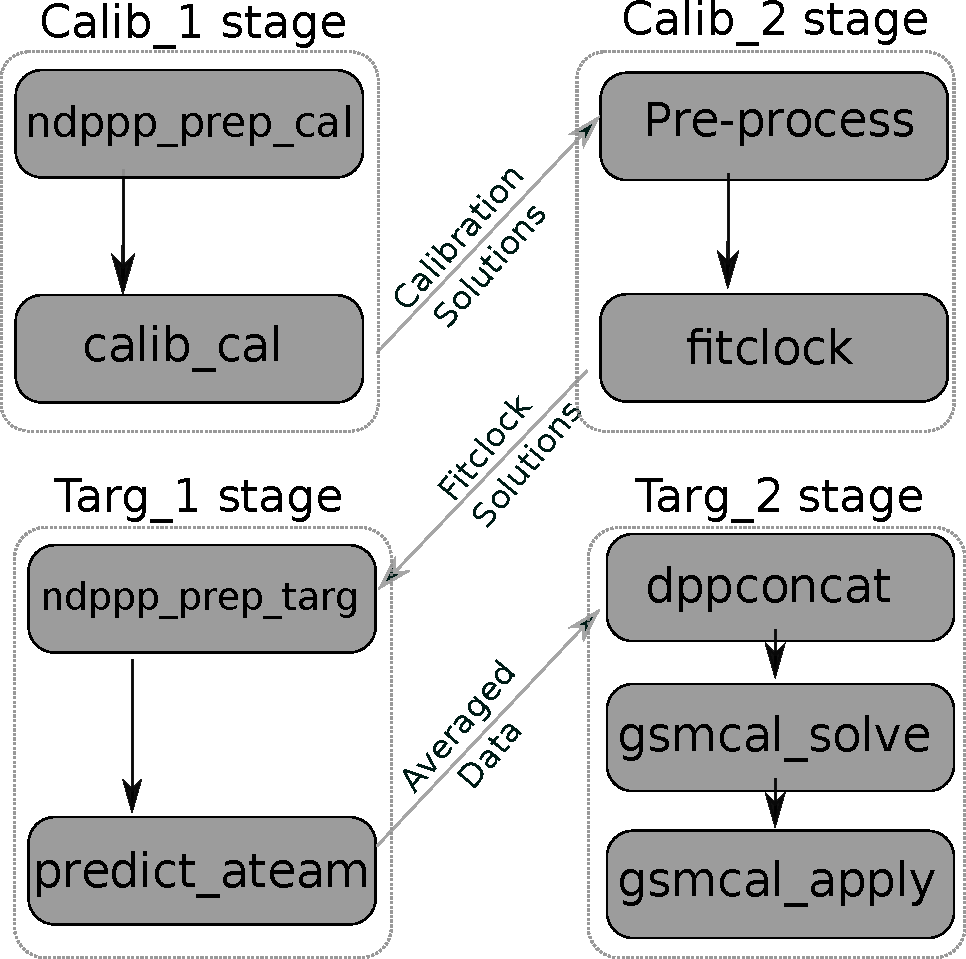
\includegraphics[width=0.5\linewidth]{ch4/figures/fig1/fig1.pdf}
      \caption[The four processing stages that make up the prefactor pipeline.]{The four processing stages that make up the prefactor pipeline. The Calibrator stages (top) process a known bright calibrator to obtain the gain for the LOFAR antennas. The Target stages (bottom) process the scientific observation to remove Direction Independent effects. The \textit{pref\_cal1} and \textit{pref\_targ1} stages are massively parallelized across nodes without the need of an interconnect. The \textit{pref\_cal2} step runs only on one node, while \textit{pref\_targ2} is parallelized on 25 nodes. As the LOFAR software does not use MPI, we can run each processing job in isolation. }
	\label{fig:ch4_four_steps_box}
\end{figure}

\begin{figure}[H]
    \centering
    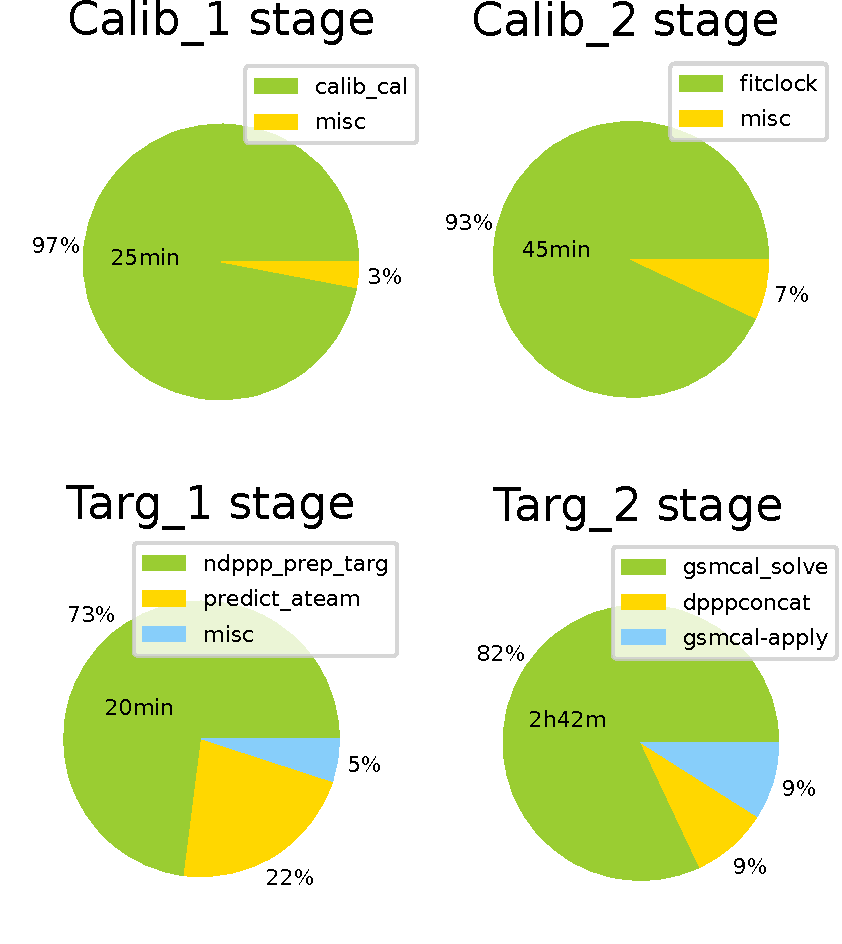
\includegraphics[width=0.5\linewidth]{ch4/figures/fig2/4pies.pdf}
      \caption[Portion of processing time taken by each step for the four prefactor stages.]{Portion of processing time taken by each step for the four prefactor stages, as reported by the Prefactor software. For each stage, the majority of processing time is spent during one or two steps. This is due to the fact that each prefactor stage also has intermediate book-keeping steps explicitly included in the pipeline. For each pipeline stage, the mean processing time for the longest running steps at SURFsara is also indicated. It should be noted that while faster, pref\_cal1 runs 10 times as many jobs as pref\_targ2. }
	\label{fig:ch4_4_steps_pies}
\end{figure}

 %\footnotetext[4]{\textit{calib\_cal} and \textit{gsmcal\_solve}}

\subsection{Performance suite}
Cluster performance is frequently monitored using utilities such as Ganglia \citep[][discussed in Section \ref{sec:ch4_related}]{ganglia}. These tools cannot access individual processes and thus cannot collect data on a per-process basis. To collect such data, each process launched by the active pipeline step needs to be profiled individually. Our utility is designed to gather such performance data.

Our monitoring package, \textit{pipeline\_collector} adds custom performance collectors (\ref{sec:ch4_customcollectors}) to the performance collection framework \textit{tcollector}. We use these collectors to monitor individual pipeline steps as defined by the user\footnote{https://gitlab.com/apmechev/pipeline\_collector.git}. The tools attach to processes launched by the pipeline and record performance data at a one second interval. This sampling frequency is at high enough resolution to detect trends and anomalies in hardware utilization, and still result in a reasonable database size. The performance data is uploaded to a remote time series database, OpenTSDB \citep{opentsdbsite}. Details on the data collection can be found in  \ref{sec:ch4_appendix1}.

\subsubsection{Performance API}\label{sec:ch4_papi2}

The time-series database is also used to collect low-level CPU information for each process. This information is collected by the PAPI interface (discussed in Section \ref{sec:ch4_related}). This was done through the papiex utility\footnote
{Available at https://bitbucket.org/minimalmetrics/papiex-oss} \citep{papiex}. This utility records the CPU's internal performance counters. A CPU's performance counters record information on how efficiently the software uses the CPU's resources. The results from this test are detailed in Section \ref{sec:ch4_PAPI}.

\subsection{Test Hardware}

In order to study the effect of different hardware configurations on the performance of LOFAR processing, the \textit{prefactor} pipeline was run on four different sets of hardware. The four machines tasked with processing LOFAR data comprised nodes at three computational clusters and a personal computer. The tests were run while the systems were idle to make sure there is no interference of other software with the LOFAR processing. Table \ref{tab:ch4_nodes} details the specifics of the four test machines.

 \begin{table}
     \begin{center} 
\resizebox{\textwidth}{!}{
  \begin{tabular}{ l | c | c | c | c | c | c }
    \hline
    Location & CPU Speed (MHz) & CPU Model & Micro-architecture & Cache Size & RAM Speed\footnotemark & Disk Speed\footnotemark \\ \hline
    \hline
    Leiden & 2200 & E5-4620 & Sandy Bridge & 16 MB  & 1.4 GB/s & 99.7 MB/s \\ \hline
    SURFsara & 2500 & E5-2680 & Sandy Bridge & 30 MB  & 2.5 GB/s & 65.4 MB/s \\ \hline
    Hatfield &  2900 & E5-2660 & Sandy Bridge  & 20 MB   & 2.4 GB/s & 155 MB/s\\ \hline
    Laptop & 3300 & E3-1505M & Skylake &  8 MB  & 4.7 GB/s & 822 MB/s\\ \hline
    \hline
  \end{tabular}}
  
         \caption[Hardware specifications of the four test machines.]{CPU, Cache, RAM and Storage specifications of the four test machines. The tested machines span a factor of 1.5x in CPU speed, 4x in cache and RAM Speed and $~$10x in Disk speed.\label{tab:ch4_nodes}}
  \end{center}
 \end{table}


